% Created by tikzDevice version 0.12 on 2019-04-30 13:33:07
% !TEX encoding = UTF-8 Unicode
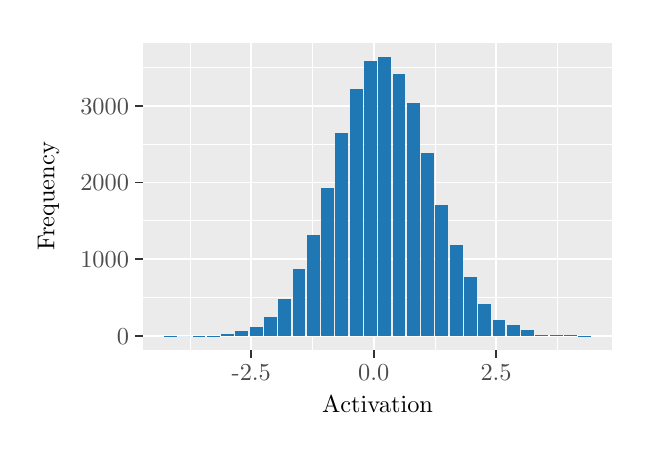
\begin{tikzpicture}[x=1pt,y=1pt]
\definecolor{fillColor}{RGB}{255,255,255}
\path[use as bounding box,fill=fillColor,fill opacity=0.00] (0,0) rectangle (216.81,144.54);
\begin{scope}
\path[clip] (  0.00,  0.00) rectangle (216.81,144.54);
\definecolor{drawColor}{RGB}{255,255,255}
\definecolor{fillColor}{RGB}{255,255,255}

\path[draw=drawColor,line width= 0.6pt,line join=round,line cap=round,fill=fillColor] (  0.00,  0.00) rectangle (216.81,144.54);
\end{scope}
\begin{scope}
\path[clip] ( 41.55, 28.07) rectangle (211.31,139.04);
\definecolor{fillColor}{gray}{0.92}

\path[fill=fillColor] ( 41.55, 28.07) rectangle (211.31,139.04);
\definecolor{drawColor}{RGB}{255,255,255}

\path[draw=drawColor,line width= 0.3pt,line join=round] ( 41.55, 46.98) --
	(211.31, 46.98);

\path[draw=drawColor,line width= 0.3pt,line join=round] ( 41.55, 74.72) --
	(211.31, 74.72);

\path[draw=drawColor,line width= 0.3pt,line join=round] ( 41.55,102.46) --
	(211.31,102.46);

\path[draw=drawColor,line width= 0.3pt,line join=round] ( 41.55,130.20) --
	(211.31,130.20);

\path[draw=drawColor,line width= 0.3pt,line join=round] ( 58.69, 28.07) --
	( 58.69,139.04);

\path[draw=drawColor,line width= 0.3pt,line join=round] (102.92, 28.07) --
	(102.92,139.04);

\path[draw=drawColor,line width= 0.3pt,line join=round] (147.16, 28.07) --
	(147.16,139.04);

\path[draw=drawColor,line width= 0.3pt,line join=round] (191.39, 28.07) --
	(191.39,139.04);

\path[draw=drawColor,line width= 0.6pt,line join=round] ( 41.55, 33.12) --
	(211.31, 33.12);

\path[draw=drawColor,line width= 0.6pt,line join=round] ( 41.55, 60.85) --
	(211.31, 60.85);

\path[draw=drawColor,line width= 0.6pt,line join=round] ( 41.55, 88.59) --
	(211.31, 88.59);

\path[draw=drawColor,line width= 0.6pt,line join=round] ( 41.55,116.33) --
	(211.31,116.33);

\path[draw=drawColor,line width= 0.6pt,line join=round] ( 80.81, 28.07) --
	( 80.81,139.04);

\path[draw=drawColor,line width= 0.6pt,line join=round] (125.04, 28.07) --
	(125.04,139.04);

\path[draw=drawColor,line width= 0.6pt,line join=round] (169.27, 28.07) --
	(169.27,139.04);
\definecolor{fillColor}{RGB}{31,120,180}

\path[fill=fillColor] ( 49.27, 33.12) rectangle ( 53.91, 33.14);

\path[fill=fillColor] ( 54.43, 33.12) rectangle ( 59.07, 33.12);

\path[fill=fillColor] ( 59.59, 33.12) rectangle ( 64.24, 33.17);

\path[fill=fillColor] ( 64.75, 33.12) rectangle ( 69.40, 33.23);

\path[fill=fillColor] ( 69.91, 33.12) rectangle ( 74.56, 33.67);

\path[fill=fillColor] ( 75.07, 33.12) rectangle ( 79.72, 34.95);

\path[fill=fillColor] ( 80.24, 33.12) rectangle ( 84.88, 36.47);

\path[fill=fillColor] ( 85.40, 33.12) rectangle ( 90.04, 39.94);

\path[fill=fillColor] ( 90.56, 33.12) rectangle ( 95.20, 46.65);

\path[fill=fillColor] ( 95.72, 33.12) rectangle (100.37, 57.44);

\path[fill=fillColor] (100.88, 33.12) rectangle (105.53, 69.56);

\path[fill=fillColor] (106.04, 33.12) rectangle (110.69, 86.65);

\path[fill=fillColor] (111.20, 33.12) rectangle (115.85,106.31);

\path[fill=fillColor] (116.37, 33.12) rectangle (121.01,122.40);

\path[fill=fillColor] (121.53, 33.12) rectangle (126.17,132.55);

\path[fill=fillColor] (126.69, 33.12) rectangle (131.33,134.00);

\path[fill=fillColor] (131.85, 33.12) rectangle (136.50,127.95);

\path[fill=fillColor] (137.01, 33.12) rectangle (141.66,117.49);

\path[fill=fillColor] (142.17, 33.12) rectangle (146.82, 99.27);

\path[fill=fillColor] (147.33, 33.12) rectangle (151.98, 80.44);

\path[fill=fillColor] (152.50, 33.12) rectangle (157.14, 65.93);

\path[fill=fillColor] (157.66, 33.12) rectangle (162.30, 54.56);

\path[fill=fillColor] (162.82, 33.12) rectangle (167.46, 44.79);

\path[fill=fillColor] (167.98, 33.12) rectangle (172.63, 39.00);

\path[fill=fillColor] (173.14, 33.12) rectangle (177.79, 36.94);

\path[fill=fillColor] (178.30, 33.12) rectangle (182.95, 35.36);

\path[fill=fillColor] (183.46, 33.12) rectangle (188.11, 33.64);

\path[fill=fillColor] (188.63, 33.12) rectangle (193.27, 33.48);

\path[fill=fillColor] (193.79, 33.12) rectangle (198.43, 33.31);

\path[fill=fillColor] (198.95, 33.12) rectangle (203.59, 33.23);
\end{scope}
\begin{scope}
\path[clip] (  0.00,  0.00) rectangle (216.81,144.54);
\definecolor{drawColor}{gray}{0.30}

\node[text=drawColor,anchor=base east,inner sep=0pt, outer sep=0pt, scale=  0.88] at ( 36.60, 30.09) {0};

\node[text=drawColor,anchor=base east,inner sep=0pt, outer sep=0pt, scale=  0.88] at ( 36.60, 57.82) {1000};

\node[text=drawColor,anchor=base east,inner sep=0pt, outer sep=0pt, scale=  0.88] at ( 36.60, 85.56) {2000};

\node[text=drawColor,anchor=base east,inner sep=0pt, outer sep=0pt, scale=  0.88] at ( 36.60,113.30) {3000};
\end{scope}
\begin{scope}
\path[clip] (  0.00,  0.00) rectangle (216.81,144.54);
\definecolor{drawColor}{gray}{0.20}

\path[draw=drawColor,line width= 0.6pt,line join=round] ( 38.80, 33.12) --
	( 41.55, 33.12);

\path[draw=drawColor,line width= 0.6pt,line join=round] ( 38.80, 60.85) --
	( 41.55, 60.85);

\path[draw=drawColor,line width= 0.6pt,line join=round] ( 38.80, 88.59) --
	( 41.55, 88.59);

\path[draw=drawColor,line width= 0.6pt,line join=round] ( 38.80,116.33) --
	( 41.55,116.33);
\end{scope}
\begin{scope}
\path[clip] (  0.00,  0.00) rectangle (216.81,144.54);
\definecolor{drawColor}{gray}{0.20}

\path[draw=drawColor,line width= 0.6pt,line join=round] ( 80.81, 25.32) --
	( 80.81, 28.07);

\path[draw=drawColor,line width= 0.6pt,line join=round] (125.04, 25.32) --
	(125.04, 28.07);

\path[draw=drawColor,line width= 0.6pt,line join=round] (169.27, 25.32) --
	(169.27, 28.07);
\end{scope}
\begin{scope}
\path[clip] (  0.00,  0.00) rectangle (216.81,144.54);
\definecolor{drawColor}{gray}{0.30}

\node[text=drawColor,anchor=base,inner sep=0pt, outer sep=0pt, scale=  0.88] at ( 80.81, 17.06) {-2.5};

\node[text=drawColor,anchor=base,inner sep=0pt, outer sep=0pt, scale=  0.88] at (125.04, 17.06) {0.0};

\node[text=drawColor,anchor=base,inner sep=0pt, outer sep=0pt, scale=  0.88] at (169.27, 17.06) {2.5};
\end{scope}
\begin{scope}
\path[clip] (  0.00,  0.00) rectangle (216.81,144.54);
\definecolor{drawColor}{RGB}{0,0,0}

\node[text=drawColor,anchor=base,inner sep=0pt, outer sep=0pt, scale=  0.88] at (126.43,  5.50) {Activation};
\end{scope}
\begin{scope}
\path[clip] (  0.00,  0.00) rectangle (216.81,144.54);
\definecolor{drawColor}{RGB}{0,0,0}

\node[text=drawColor,rotate= 90.00,anchor=base,inner sep=0pt, outer sep=0pt, scale=  0.88] at (  9.62, 83.56) {Frequency};
\end{scope}
\end{tikzpicture}
